% BE�LL�T�SOK - JOBB NEM V�LTOZTATNI

\documentclass[final]{ubb_dolgozat}
\usepackage{definitions}
\usepackage{pdfpages}
\usepackage{listings}

\newcommand{\pdf}[1]{pythonCodes/#1.pdf}
%%


% milyen nyelveken akarunk forr�sk�dot megjelen�teni
\lstloadlanguages{C, C++, Python}

% ezt be lehet tenni MINDEGYIK megjelen�tend� k�d el�.
\lstset{language=Python}


%% MELYIK �VBEN ADJUK LE
\submityear{%
2015
}
%% MELYIK H�NAPBAN ADJUK LE
\submitmonthHU{%
J�lius
}
\submitmonthRO{%
Iulie
}
\submitmonthEN{%
July
}

\titleHU{%
Forgalmi t�bl�k felismer�se
}
\titleEN{%
Road sign recognition
}

\titleRO{%
Recunoa\c{s}terea semnelor de circula\c{t}ie
}

\author{%
Szabo �gnes-Ter�z
}

%%
\tutorHU{%
Csat� Lehel\\
 {\large Babe\c{s}--Bolyai Tudom�nyegyetem,\\
 Matematika �s Informatika Kar}
}

%%
\tutorRO{%
Csat� Lehel\\
 {\large Universitatea Babe\c{s}--Bolyai,\\
 Facultatea de Matematic\u{a} \c{s}i Informatic\u{a} }%
}
%%
\tutorEN{%
Csat� Lehel
 {\large Babe\c{s}--Bolyai University,\\
 Faculty of Mathematics and Informatics}
}


%\includeonly{bevezet}


\begin{document}

%% ABSTRAKT
\begin{abstractEN} % ANGOL V�LTOZAT

\vfill
I work on a system which as an input gets a sound file, proccesses it, analyzes it, and as an output generates a sheet music, which contains the detected music notes from the sound file.


This work is the result of my own activity. I have neither given nor received unauthorized assistance on this work.

\vfill

\end{abstractEN}


% ez a c�moldal r�sze
\maketitle
%% 

% a dolgozat tartalomjegyz�ke -- ez automatikusan gener�l�dik a STRUKT�RA alapj�n.
{ \baselineskip 1ex
  \parskip 1ex
  \tableofcontents
}


%%%%%%%%%%%%%%%%%%%%%%%%%%%%%%%%%%%%%%%%%%%%%%%%%%%%%%%%%%%
%%%%%%%%%%         a dolgozat tartalma         %%%%%%%%%%%%



% a bevezet� fejezet FILE-ja.
%!TEX root = dolgozat.tex
%%%%%%%%%%%%%%%%%%%%%%%%%%%%%%%%%%%%%%%%%%%%%%%%%%%%%%%%%%%%%%%%%%%%%%%
\chapter{Introduction}\label{ch:INTRO}
%%%%%%%%%%%%%%%%%%%%%%%%%%%%%%%%%%%%%%%%%%%%%%%%%%%%%%%%%%%%%%%%%%%%%%%

\section{Goal}\label{sec:INTRO:goal}

 ide egy altalanos mondat I am developing a system that can detect and recognise road signs on pictures taken in real life enviroment. There are many similar systems, but the robust cost-effective solution is still an active research subject. Since there are numerous types of traffic signs and many of them are similar to one another, the task of classifying them is challenging. The recognizability of the road signs is also affected by the following things: luminous intensity, shading, partial coverage, and other obstacles.

My goal is to make a fast and efficient system. This can also be a first step to developing a system that can recognise traffic signs on video files and on live camera feed.

\section{Implementation}\label{sec:INTRO:implement}

This system recognises road signs with machine learning algorithms.I use artificial neural networks, a subclass of S L. I use supervised learning, since I know the desired outcome of an input(the road sign's class), more precisly artificial neural networks.

When an application is placed in real enviroment it is crucial for it to be reliable. Wrongly identifying a road sign can have fatal consequences.

Because traffic signs can change with time it is important that the designed system can accomodate to these changes, without the need to change it to the core. Artificial neural networks are perfect for this, because if the data changes it is enough to perform the learning process again, there is no need do change the code.
%!TEX root = dolgozat.tex
%%%%%%%%%%%%%%%%%%%%%%%%%%%%%%%%%%%%%%%%%%%%%%%%%%%%%%%%%%%%%%%%%%%%%%%
\chapter{Road signs}\label{ch:SIGNS}
%%%%%%%%%%%%%%%%%%%%%%%%%%%%%%%%%%%%%%%%%%%%%%%%%%%%%%%%%%%%%%%%%%%%%%%

\section{What are road signs}\label{sec:SIGNS:whatAreThey}

Traffic signs control the flow of traffic, warn the driver of hazards ahead, guide the driver to their destination, and inform them of roadway services. There are three basic types of traffic signs all with different shapes: 

- signs that give orders, circular

- warning signs, triangular

- signs that give information, rectangular

The stop sign is an exception, it is an octagon.


A further guide to the function of a sign is its colour. The colors used are red, white, black, and blue. %All triangular signs are red.

Most of the road signs are composed of two parts: a solid band on the outside and the inside figure or number. The inside symbol is usually black. 

\section{Charateristics}\label{sec:SIGNS:character}

\section{Data set}\label{sec:SIGNS:dataSet}

\subsection{Training data}

I used ... . It contains 1213 training images, their size varies from 16x16 to 128x128 pixels, they appear in every perspective and under every lighting condition. The images are divided in 43 categories based on the containd traffic signs.

Altough there is a large amount of training images, they are not devided equally among categories. This                       makes it difficult for the network to learn the specifics of the classes that contain small amounts of images.

I try to equalize the number of training images by generating more images into that category. The original training set contains images that completely contain the traffic sign. Since my purpose is to recognise partially visible road signs too, I generate new images from the old ones by cutting out 70-80\% of them.

\begin{figure}
\centering

\includegraphics{trainingImage}
\includegraphics{trainingImage2}
\caption{Example of the training images}

\label{fig:trainingImage}
\end{figure}

\subsection{Test data}

There are 900 test images, containing zero to six traffic signs. They are significantly larger pictures: 1360 x 800 pixels. On the \ref{fig:trainingImage} figure is an example of the test images, that contains two road sings.

\begin{figure}[h]
\centering

\includegraphics[scale=0.4]{testImage}
\caption{An example of the test images}

\label{fig:trainingImage}
\end{figure}


%!TEX root = minta_dolgozat.tex
%%%%%%%%%%%%%%%%%%%%%%%%%%%%%%%%%%%%%%%%%%%%%%%%%%%%%%%%%%%%%%%%%%%%%%%
\chapter{Darabolás}\label{ch:SEGMENT}
%%%%%%%%%%%%%%%%%%%%%%%%%%%%%%%%%%%%%%%%%%%%%%%%%%%%%%%%%%%%%%%%%%%%%%%

Annak érdekében, hogy megtaláljunk egy forgalmi táblát egy képen, szegmentációt alkalmaztam. A szegmentáció az a folyamat, amikor kisebb képeket vágunk ki egy nagyobb képből. \cite{7}

Több különböző módszer létezik a szegmentálás végrehajtására. Az általam alkalmazott véletlenszerű kiválasztáson alapszik. Véletlenszerű téglalapokat generálok és vágom ezeket ki az eredeti képből.

Mivel a valós környezetből vett képek több forgalmi táblát is tartalmazhatnak, fontos hogy az egész képet bejárják ezek a darabok. Az által hogy nagy számban generálok ilyen darabokat, biztosítom, hogy nagy valószínűséggel megtaláljam a képen levő forgalmi táblákat. A táblák mérete is változik attól függően, hogy milyen távolságra van a fényképezőtől, ezért arra is figyelnem kellett, hogy a kivágott darabok mérete széles tartományban mozogjon.

Az által, hogy véletlenszerűen választom ki a vizsgálandó részeket az eredeti képből, ezeknek nagy része olyan kép lesz, ami nem tartalmaz forgalmi táblát vagy csak részlegesen fogja azt tartalmazni. Ez az oka annak, hogy a neurális háló akkor is megfelelően kell osztályozza a táblát ha csak 70-80\% látszik belőle.

\begin{figure}[h]
\centering

\includegraphics[scale=0.3]{images/testImage2}
\caption{Szegmentálás előtti kép}

\label{fig:testImage2}
\end{figure}

\makeatletter
    \setlength\@fptop{0\p@}
\makeatother

\begin{figure}[htbp]
\centering

\includegraphics[scale=1]{images/segments}
\caption{Példa szegmentálás utáni képekre}

\label{fig:segments}
\end{figure}
%!TEX root = dolgozat.tex
%%%%%%%%%%%%%%%%%%%%%%%%%%%%%%%%%%%%%%%%%%%%%%%%%%%%%%%%%%%%%%%%%%%%%%%
\chapter{Képek előfeldolgozása}\label{ch:PREPROC}
%%%%%%%%%%%%%%%%%%%%%%%%%%%%%%%%%%%%%%%%%%%%%%%%%%%%%%%%%%%%%%%%%%%%%%%

\begin{osszefoglal}
Annak érdekében, hogy egyszerűsítsem a bevitt adatokat, előfeldolgozást végzek a képeken a színük alapján. A neurális háló a pixelek szürke árnyalatával dolgozik. 
A képek különböző fényviszonyok mellett készültek, ennek köszönhetően némelyik nagyon világos, mások pedig nagyon sötétek.

Megjegyzés: A képek valós környezetből származnak, így más objektumokat is tartalmazhatnak, mint például faágak.

\end{osszefoglal}

\section{Színterek}\label{sec:PREPROC:colorSpaces}

A szín a módja annak, ahogyan az emberi látórendszer a bejövő elektromágneses sugárzást értelmezi. Az a tartomány, ahol a rendszer színként érzékeli ezt a sugárzást körülbelül 400 és 830 nm-es hullámhosszak között jelentkezik (személytől függően változhat némileg) \cite{17}. 

A színterek pontosan meghatároznak színeket az érzékelhető hullámhossz tartományból. 
Arra szolgálnak, hogy könnyebben tudjuk meghatározni, létrehozni és felfogni a színeket. Egy színt általában három paraméter határoz meg. Ezek fejezik ki az adott szín helyét az illető színtérben. Különböző színtereket ismerünk, attól függően válasszuk ki a megfelelőt, hogy mire akarjuk alkalmazni \cite{4}. 






\subsection{RGB színtér}\label{sec:PREPROC:rgb}

Az RGB színtér (\ref{fig:RGBColorSpace}) egy additív színrendszer, mely a tri-kromatikus elméleten alapszik. A tri-kromatikus elmélet lényege, hogy 3 különböző szín segítségével bármilyen szín kikeverhető.  
Az RGB színtér könnyen implementálható, de nem párhuzamos az emberi látással. Az RGB színteret gyakran felhasználják számítógépes alkalmazásokhoz, mert nincs szükség transzformációra ahhoz, hogy megjelenítsük az információt. A színtér legegyszerűbb ábrázolása egy kocka, ahol a 3 tengely a piros, zöld és kék színekkel egyenértékű. 


\subsection{HSV színtér}\label{sec:PREPROC:hsv}

Ellentétben az RGB ábrázolással, a HSV színtér (\ref{fig:HSVColorSpace}) henger-koordinátákat alkalmaz. Ez az egyik leggyakoribb ábrázolási módszer. Az árnyalat(hue) az az emberi érzet, amely szerint egy szín egy másik színre vagy több szín keverékére hasonlít a piros, sárga, zöld és kék színek közül. A szín telítettsége (saturation) egy szín színessége és a fényessége közti arány. A fényesség (value-brightness) az az emberi érzet, hogy egy terület több vagy kevesebb fényt áraszt magából. 


\begin{figure}[h]
\centering

\includegraphics[scale=0.1]{RGBColorSpace}
\caption{RGB színtér}
\small forrás:\url{http://upload.wikimedia.org/wikipedia/commons/8/83/RGB_Cube_Show_lowgamma_cutout_b.png}
\label{fig:RGBColorSpace}
\end{figure}

\begin{figure}[h]
\centering

\includegraphics[scale=0.1]{HSVColorSpace}
\caption{HSV színtér}
\small forrás:\url{http://upload.wikimedia.org/wikipedia/commons/0/0d/HSV_color_solid_cylinder_alpha_lowgamma.png}
\label{fig:HSVColorSpace}
\end{figure}

\section{Megvalósítás}\label{sec:PREPROC:implement}

A forgalmi táblák figyelemfelkeltőek kell legyenek, ezért jól látható színeket használnak, mint például piros, kék, sárga, fekete és fehér.

A bemeneti képeket szín alapján szűröm, ezáltal felépítek egy új, fekete-fehér képet. Ha az árnyalat, a telítettség és a fényesség egy bizonyos intervallumban helyezkedik el, az új kép megfelelő pixelje fekete lesz, különben fehér. Ezeket az intervallumokat kísérletezéssel és a \ref{fig:colorWheel} ábra segítségével határoztam meg.

\begin{figure}[h]

\centering 
\includegraphics[scale=0.5]{ColorWheel}
\caption{Színkör}
\small forrás:\url{http://stackoverflow.com/questions/21737613/image-of-hsv-color-wheel-for-opencv}
\label{fig:colorWheel} 

\end{figure}

\begin{center}
\begin{table}[h]
\centering
\begin{tabular}{ |p{3cm}||p{3cm}|p{3cm}|p{3cm}|  }
 \hline
 Szín & Árnyalat & Telítettség & Fényesség\\
 \hline
 Piros   & 0-20, 340-360    &>0.3& >0.2\\
 Sárga &   25-60  & >0.3 & >0.2\\
 Kék & 180-270 & >0.3 & >0.2\\
 Fekete    & - & - & <0.3\\
 \hline
\end{tabular}


\caption{Elfogadási tartomány}
\label{table:1}
\end{table}
\end{center}

\section{Átméretezés}

Mivel a tanulási adatok és a teszt adatból kivágott képek mérete is változó, a képeket átméretezem 25x25 pixelre és ezzel dolgozom tovább. Ennek következtében adatvesztés és torzulás léphet fel, amikor más méretű képet méretezek át.

%!TEX root = dolgozat.tex
%%%%%%%%%%%%%%%%%%%%%%%%%%%%%%%%%%%%%%%%%%%%%%%%%%%%%%%%%%%%%%%%%%%%%%%
\chapter{Neurális hálózatok}\label{ch:INTRO}
%%%%%%%%%%%%%%%%%%%%%%%%%%%%%%%%%%%%%%%%%%%%%%%%%%%%%%%%%%%%%%%%%%%%%%%

\begin{osszefoglal}
Ebben a fejezetben megnézzük a biológiai modellt aminek a mintájára a mesterséges neuronokat létrehozták, megismerkedünk a mesterséges neuronokkal és a neurális hálókkal majd pedig megnézzük hogyan is tanulnak ezek.
\end{osszefoglal}

\section{Bevezető}
\subsection{Biológiai modell}

Az idegsejtek (neuronok) az idegrendszer alkotóelemei. A neuron jeleket fogad és ezekre megfelelő választ generál. Az emberi idegrendszer nagyon komplex műveletek elvégzésére képes rövid idő alatt. Mivel ennek analógjára hozták létre a mesterséges neurális hálókat, ezért fontos a biológiai alapok megismerése.

A \ref{fig:idegsejt} ábrán látható egy idegsejt és annak részei. A dendritek más neuronokkal állnak kapcsolatban és a bejövő információt szállítják. A beérkezett információ feldolgozását a sejtmag hajtja végre. Az idegrost egy szigetelt vezető aminek az a feladata, hogy továbbszállítsa az információt. Az axonvégek más neuronok dendritjeivel vannak kapcsolatban, a választ szállítják tovább a velük kapcsolatban levő idegsejteknek. 


\begin{figure}[h]
\centering

\includegraphics[scale=0.5]{images/idegsejt}
\caption{Idegsejt}
\small forrás:\url{http://www.clker.com/clipart-neuron.html}


\label{fig:idegsejt}
\end{figure}


\section{Mesterséges neuronok}\label{sec:INTRO:neurons}
A neuronok a neurális hálók építőkövei. 
\subsection{Szigmoid neuron}

A szigmoid neuron 0 és 1 közötti értékeket kap bementi paraméterként és létrehoz egy kimentet ugyanebben az intervallumban.

\begin{figure}[h]
\centering

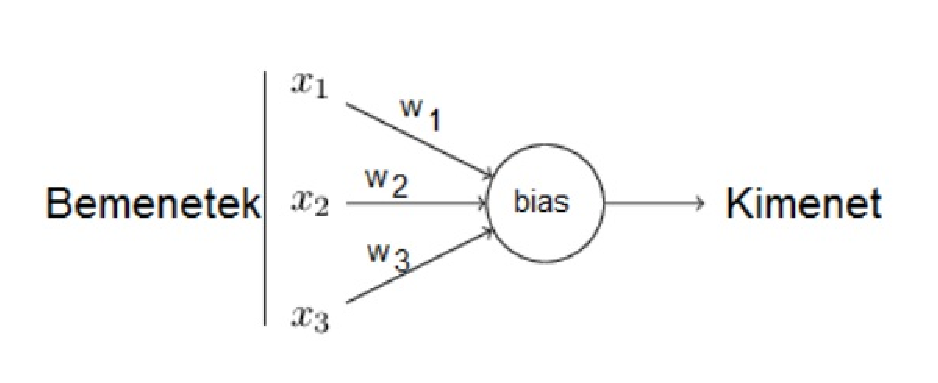
\includegraphics[scale=1]{images/neuron.eps}
\caption{Szigmoid neuron}
\small forrás:\url{http://neuralnetworksanddeeplearning.com/chap1.html}


\label{fig:neuron}
\end{figure}

Mindegyik bemenethez súlyok vannak rendelve, ami azt jelképezi, hogy az illető bemenet mennyire játszik fontos szerepet a neuron kimenetében. Minden neuronhoz tartozik továbbá egy küszöbérték, ami a kisebb rendellenességek javítására szolgál.

A szigmoid neuron kimenete a \ref{eq:1} képlettel számítható ki.

\begin{equation} \label{eq:1}
\sigma(\sum\limits_{i=1}^{n-1} w_{i}x_{i} + b)
\end{equation}

\begin{equation} \label{eq:2}
\sigma(z) = \frac{1}{1+e^{-z}}
\end{equation}

A \ref{eq:2} függvényt aktiválási függvénynek nevezik. Az aktiválási függvény szerepe, hogy a kimenetet egy adott intervallumba szorítsa. Ahogy ez az \ref{fig:sigmoidf} ábrán is látszik, a szigmoid neuron esetében ez az intervallum 0 és 1 között van. 

\begin{figure}[h]
\centering

\includegraphics[scale=0.35]{images/sigmoidf.eps}
\caption{Szigmoid függvény grafikus képe}

\label{fig:sigmoidf}
\end{figure}

A szigmoid neuron egyik tulajdonsága, hogy kis változás a súlyokban kis változást eredményez a kimenetben. Ez egyszerre előny és hátrány is. Előny, mert amikor a kimenet közel van az elvárt kimenethez, a módosítások nem eredményezik azt, hogy a kimenet túlságosan eltávolodjon az elvárttól. Hátrány, mert amikor a kimenet nagyon helytelen, mint például a tanulás elején, hosszú időbe telik a javítása \cite{5}.

\section{Neurális hálók struktúrája}\label{sec:INTRO:architecture}

A neuronokból álló hálózatokat neurális hálóknak nevezzük. A hálózat neuronjai hasonló típusú műveletet végeznek a többi neurontól függetlenül. Egy neuron sok más neuronnal áll kapcsolatban, ahogy ez a biológiai analógiából kikövetkeztethető. Tehát a neurális hálózatok olyan információfeldolgozó eszközök, amelyek párhuzamos, elosztott működésre képesek, lokális feldolgozást végző neuronokból állnak, képesek tanulni, és a megtanult információt felhasználni \cite{10}.

A neuronok egy hálózaton belül általában csak meghatározott számú neuronnal vannak összekötve, és ez a kapcsolat általában egyirányú, ezért a hálózatokat különböző rétegekre szoktuk bontani az összekötések szerint. Az egyes rétegekhez tartozó neuronok az előző réteg neuronjainak kimenetével, vagy a bemenettel, illetve a következő réteg bemenetével vannak összekötve \cite{10}.


\begin{compactenum}
	\item Bemeneti réteg: azok a neuronok találhatók itt, amelyek a bemeneti jel továbbítását végzik a hálózat felé. A legtöbb esetben nem jelöljük őket külön
	\item Rejtett réteg: a tulajdonképpeni feldolgozást végző neuronok tartoznak ide. Egy hálózaton belül több rejtett réteg is lehet
	\item Kimeneti réteg: az itt található neuronok a külvilág felé továbbítják az információt. A feladatuk ugyanaz, mint a rejtett rétegbeli neuronoké \cite{10}.
\end{compactenum}


Ennek függvényében a neuronok elhelyezkedésük alapján három csoportba sorolhatók:
\begin{compactenum}
	\item Bemeneti neuronok
	\item Rejtett neuronok
	\item Kimeneti neuronok
\end{compactenum}


A legtöbb hálózat esetében az egyes rétegek teljesen össze vannak kötve, vagyis egy réteg egy neuronjának kimenete a következő réteg összes bemenetével össze van kötve. A hálózatoknál előforduló számítások elvégzéséhez célszerűbb a hálózatokat különböző mátrixokkal jellemezni. A bemeneteket elegendő egy darab vektorba rendezve ábrázolni, ez N bemenet esetén egy N-es vektort jelent. Az egyes rétegek közötti súlyokat hasonlóan a bemenetekhez mátrixokba szoktuk rendezni. Ez a következőképpen néz ki: ha az l. rétegben n darab neuron van az l+1. rétegben pedig m, akkor a köztük lévő súlyok száma n x m. Ez mátrixba rendezve egy m x n-es mátrixot jelent, amelynek oszlopai az l. réteg neuronjait, sorai az l+1. réteg neuronjait reprezentálják \cite{10}. 

\begin{figure}[h]
\centering

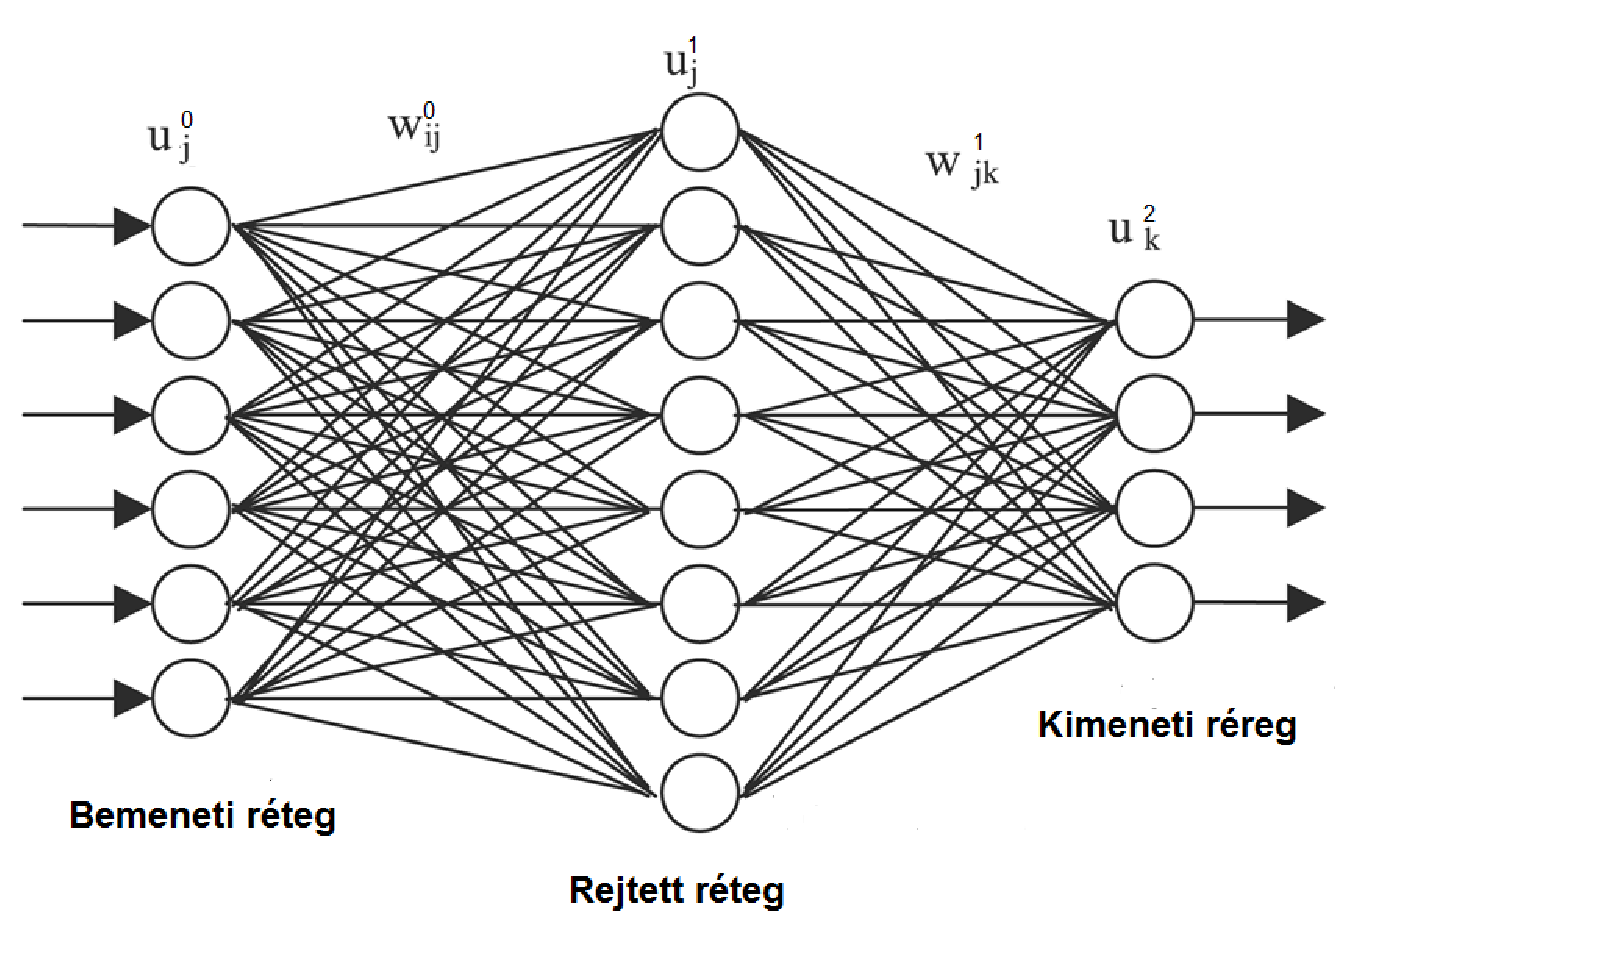
\includegraphics[scale=0.5]{images/net.eps}
\caption{Egyszerű neurális háló}

\label{fig:net}
\end{figure}

A \ref{fig:net} ábrán egy egyszerű szigmoid neuronokból álló neurális háló látható. A súlyvektorok mérete már ennél a kis példánál is viszonylag nagy, ezért egy nagy hálónál ezek az értékek jelentősen megnőnek.


Olyan neurális hálót használtam, amelynek 625 bemenete és 43 kimenete van. A bemeneti neuronok a kép egy pixelének szürke árnyalatát tartalmazzák. A kimenetek száma megegyezik a forgalmi táblák osztályainak a számával. 

\section{Sztochasztikus gradiens csökkentés}\label{sec:INTRO:graddesc}

Annak érdekében, hogy a súlyokat és küszöbértékeket a kimenetnek az elvárt eredménytől való eltérése függvényében tudjam módosítani, a sztochasztikus gradiens csökkentést alkalmaztam. Ez a gradiens csökkentés egyszerűsített változata. Gradiens csökkentéssel a teljes tanítási adathalmazra számolja a hiba értékét, míg a sztochasztikus gradiens csökkentés közelíti a hibát egy bizonyos számú véletlenszerűen kiválasztott adat alapján. Minél nagyobb ez a szám, a közelítés pontossága annyival jobb lesz, de mivel nem a teljes adathalmazzal dolgozik, ezért gyorsabb lesz.

A \ref{eq:3} egyenlet a négyzetes hibafüggvény. \textit{n} a bemeneti tanítási adatok száma, \textit{y(x)} az \textit{x} bemenetre a háló által generált kimenet és \textit{a} az elvárt kimenet az \textit{x} bemenetre. Amikor az elvárt és a kiszámított kimenet közel van egymáshoz, a hiba kicsi lesz. Mivel a célom, hogy a kiszámított kimenet az elvárt kimenetet közelítse meg minél jobban, ezt a hibát kell minimalizálnom. Ennek érdekében bevezetem a  $\Delta C$-vel jelölt gradiensét a hibafüggvénynek. A gradiens értékét a \ref{eq:6} képlettel lehet kiszámítani.

\begin{equation} \label{eq:3}
\ C = \frac{1}{2n}\sum\nolimits_{x} \|y(x)-a(x)\|^2
\end{equation}

\begin{equation} \label{eq:6}
\ \Delta C = (\frac{\partial C}{\partial w_{i}},\frac{\partial C}{\partial b_{j}})^T
\end{equation}

A hiba csökkentése érdekében ismételtem alkalmaztam a \ref{eq:4} és a \ref{eq:5} szabályokat a súlyokra és küszöbértékekre. $\eta$ a tanítási ráta. Ez egy kicsi érték kell legyen, de nem túl kicsi, mert akkor a tanulási folyamat túl lassú lenne.

\begin{equation} \label{eq:4}
\ w_{i} \rightarrow w_{i} - \eta\frac{\partial C}{\partial w_{i}} 
\end{equation}

\begin{equation} \label{eq:5}
\ b_{j} \rightarrow b_{j} - \eta\frac{\partial C}{\partial b_{j}} 
\end{equation}


\section{Backpropagation}\label{sec:INTRO:backprop}


A backpropagation algoritmus arra szolgál, hogy a háló súlyait és küszöbértékeit úgy állítsa be, hogy a kimenet megközelítse minél jobban az elvárt kimenetet.

A \ref{eq:7} egyenletben $z^l$ a súlyozott bementi vektor az l-edik rétegben. Ahogy a \ref{eq:8} egyenletben látható, a kimeneti vektor egy rétegben az előző réteg kimenetének használatával számolható ki, vagyis az információ továbbításával. A háló kimenetének kiszámítása után a \ref{eq:9}-es egyenlet segítségével lehet kiszámolni az utolsó réteg hibáját, ahol \textit{L} a rétegek számát jelöli, \textit{$\Delta_aC$} pedig a $\frac{\partial C}{\partial a_j^L}$ parciális deriváltakat tartalmazó vektor.


Maga a backpropagation a \ref{eq:10} képlet segítségével történik minden \textit{l} rétegre, \textit{L-1}-től 2-ig.

\begin{equation} \label{eq:7}
\ z^l = (w^la^{l-1} + b^l) 
\end{equation}

\begin{equation} \label{eq:8}
\ a^l = \sigma(z^l) 
\end{equation}

\begin{equation} \label{eq:9}
\ \delta^L = \Delta_a C \circ \sigma'(z^L)
\end{equation}

\begin{equation} \label{eq:10}
\ \delta^l = ((w^{l+1})^T \delta^{l+1}) \circ \sigma'(z^l)
\end{equation}

\chapter{Az algoritmus} \label{algorihm}

 
\begin{algorithm}
\caption{Backpropagation}
\label{pseudoPSO}
\begin{algorithmic}[1]
\State Súlyok és küszöbértékek inicializálása véletlenszerű adatokkal
\For{Minden ciklus $i$}
    \State Tanulási adatok összekeverése
    \For{Minden batch $j$}
    	\For{Minden $d$ tanulási adatra a $j$ batch-ből }
		    \State Minden réteg kimenetének kiszámítása a \ref{eq:2} egyenlet segítségével a bemenettől a kimenet felé
		    \State Kimenet hibájának kiszámítása a \ref{eq:9} egyenlet segítségével
		    \State Minden neuron hibájának kiszámítása a kimenettől a bemenet felé haladva a a \ref{eq:10} egyenlet segítségével
		\EndFor
		\State $d$ tanulási adatra számított hibák összegzése 
		\State Súlyok és küszöbértékek módosítása felhasználva a hibák összegét a \ref{eq:4} és \ref{eq:5} egyenlet segítségével
    \EndFor
\EndFor
\end{algorithmic}
\end{algorithm}

 Ahhoz, hogy a háló tanulni tudjon, fontos az, hogy a súlyokat és küszöbértékeket megfelelően kicsi számokkal inicializáljuk. Ezt úgy valósítottam meg, hogy a 0 és 1 között véletlenszerűen generált számot elosztottam 3000-el.
 
 A batch-ben egyidőben jelen levő adatok minél változatosabbak kell legyenek, annak érdekében hogy tanulás közben egy időben figyelembe vegye a különböző osztályok tulajdonságait. Ezért van szükség az adatok összekeverésére. A beolvasás sorban történik, vagyis az azonos osztályba tartozóak egymás után fognak szerepelni. Ha ebben a sorrendben kerülnének be a batch-be, akkor a háló először megpróbálná megtanulni az egyik osztály tulajdonságait, utána pedig sorban a következőkét. Az adatok keverésével ezt kerülöm el \cite{5}.


\appendix
\include{programok}


{ \renewcommand{\baselinestretch}{0.8}\normalsize %
  \setlength{\itemsep}{-2.4mm}
  \setlength{\bibspacing}{0.67\baselineskip}
  \bibliographystyle{abbrvnat_hu}
  \bibliography{konyveszet}
}



\end{document}
